\section{Validation against the record's outcomes}\label{sec:validation}

A measure is worth the outcomes it can be tested against. The record
supplies four that are dated and high-stakes: whether an application
reached registration, whether a registered mark's owner proved continued
use at year six, whether the owner patents, and whether the owner
appears in SEC reporting. This section reports what each axis predicts
at each, under the design the corpus supports --- class-by-year fixed
effects, drafting and filer controls, owner-clustered errors --- and
states, for each result, whether it survives the alternative
constructions of Section~\ref{sec:robust}. What the results say about
pioneering is the subject of the companion paper.

\subsection{Registration rises with atypicality and is nearly flat in
lead}\label{sec:reg_rates}\label{sec:val_registration}

Figure~\ref{fig:regdeciles} gives the registration rate by decile of
each axis, deciles cut within Nice class and filing year. On atypicality
the rate rises from 56.0\% in the least atypical decile to 59.1\% in the
ninth and turns down to 58.3\% in the most atypical. On lead the range
across deciles is 0.9 points: filings written in language their class
was moving toward register at nearly the same rate as filings written in
language it was leaving, though a linear fit tilts slightly upward.

\begin{figure}[h]\centering
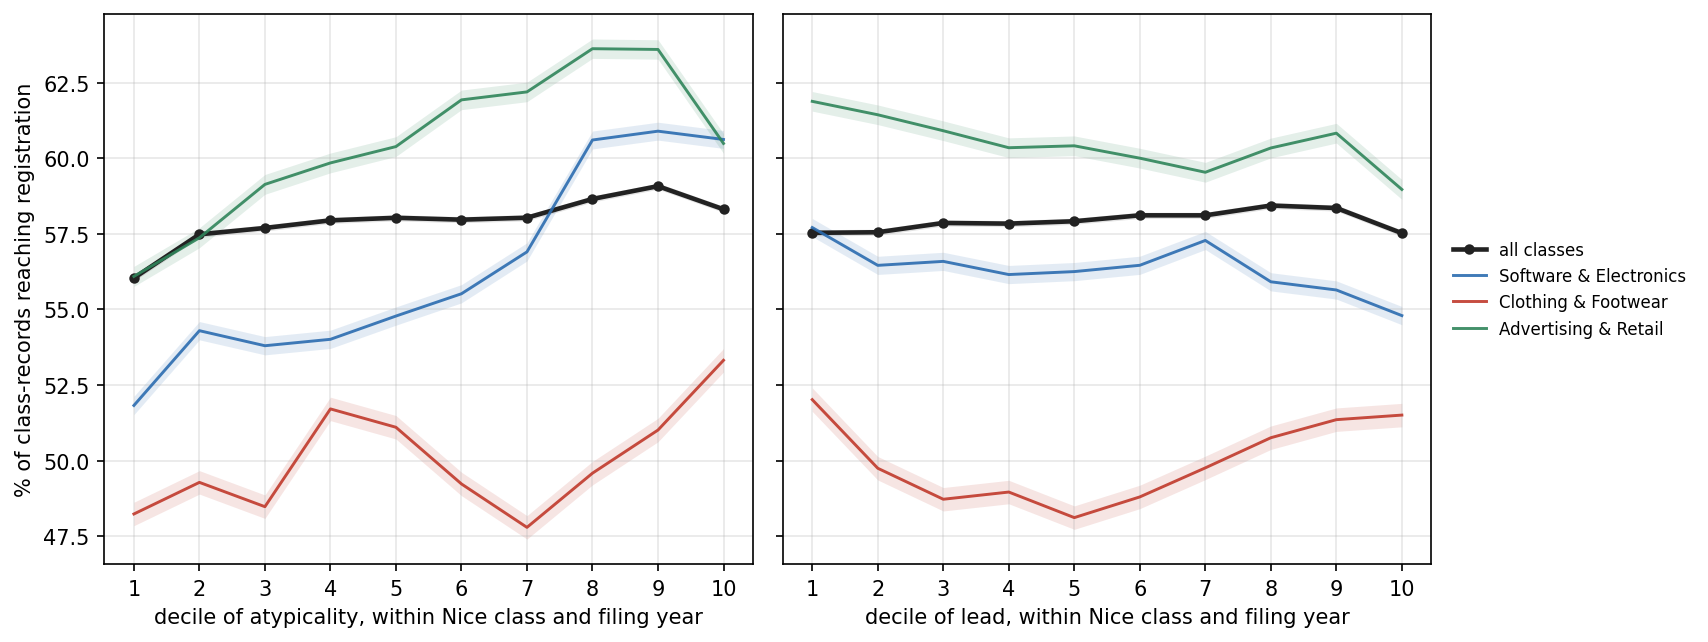
\includegraphics[width=\textwidth]{results/fig_registration_deciles.png}
\caption{Share of class-records reaching registration, filings
1995--2018, by decile of atypicality (left) and of lead (right), deciles
cut within Nice class and filing year; $n = 9{,}024{,}532$ scored
class-records. The black line pools all 45 classes; the colored lines
are three named classes. The grey band is a 95\% binomial interval on
the pooled line.}
\label{fig:regdeciles}
\end{figure}

The flatness of lead at this step has a mechanical reading worth
stating: lead is computed from the five years of filings \emph{after}
the filing date, which had not happened when the examiner acted. No
participant in prosecution could observe the quantity. Atypicality's
past-facing half, by contrast, is exactly what an examiner steeped in
the class's usual language experiences, and it is the axis registration
responds to.

Two cautions on the level. First, registration is mostly a measure of
the applicant's own follow-through: nine in ten failed applications die
by inaction, and only 4.3\% are removed adversarially
(Table~\ref{tab:funnel}). Second, the shape depends on the cut. On the
pooled distribution, restricted to debut filings, the atypicality curve
is an inverse-U with a deeper conventional tail (46.6\% at the bottom,
about 58\% in the middle, 53.4\% at the top); the within-cell profile of
Figure~\ref{fig:regdeciles} is the cleaner statement, and on it the
conventional tail, not the atypical one, is the penalized end. Both
shapes reward a middling distance from the class's language --- the
pattern audience-conformity research predicts for evaluators
\citep{Zuckerman1999, Hsu2006, Zhao2017}, here from an examiner at
census scale. Unfamiliarity alone cannot produce it, since completion
falls at both ends, and the curvature is specific to the unsigned axis
(Supplementary Material, \S S1, carries the debut profiles, the
counsel-vs-self-filed split, and refiling behaviour).

\subsection{The five-year proof: leading marks fail it more
often}\label{sec:gate}\label{sec:val_gate}

The question here is about products that entered commerce: given that a
product was brought to market, does the language of its first
description predict whether it was still there five years on?
Registration is the record's marker of entry, so the analysis conditions
on it. An application that never registered left the record, nine times
in ten, by the applicant's own inaction, before any product met a
customer; pooling those applications in would change the question into
one about everyone who considered launching. Refiling does not
undermine the conditioning: 3.6\% of abandoned applications are refiled
within six years, refiled cases are 1.1\% of this sample and fail at
nearly the sample rate, and the headline contrast is $+2.25$pp with
them and without them. The supplementary material (\S S4) reports the
pooled analysis for a skeptical reader; its gradients are attenuated and in
places reversed, because the registration step's shape is stamped onto
every later outcome.

Marks written in language their industry subsequently moved toward fail
the five-year proof more often than marks written in language it was
moving away from. Within Nice class and registration year, controlling
for whether the filer drafted the mark themselves or hired counsel, and
for the length of the description, registrations in the most leading
fifth of lead fail $1.4$ points more often (53.3\%) than those in the
most lagging fifth (51.9\%; $t = 8.3$, Table~\ref{tab:gate_lpm}). The
primary estimates come from a linear probability model on 3.10 million
unique registrations with lead quintiles cut within Nice class and
registration year, class$\times$registration-year fixed effects,
controls for counsel of record, intent-to-use basis, log description
length, log owner filing volume, owner domicile and foreign filing
basis, and standard errors clustered on 1.27 million normalized owners.

\begin{table}[h]\centering\small
\caption{Failure at the five-year proof of continued use and lead:
design-based estimates. LPM of event-dated failure on
within-class$\times$registration-year lead quintiles (Q1 omitted),
unique serials, registrations 2002--2018. Failure is a dated
cancellation for non-use at registration age 4.0--8.5 years, under \S8
or, for Madrid \S66(a) registrations, \S71. All specifications include
class$\times$registration-year fixed effects; controls are counsel of
record, intent-to-use basis, log goods/services length, log owner
filing count, owner domicile (US, CN), and foreign basis (\S44(e),
\S66(a)). Base failure rate 52.3\%. The same estimates are the main
result of a companion paper on pioneering.}
\label{tab:gate_lpm}
\begin{tabular}{llrrr}
\toprule
Sample & Specification & Q5$-$Q1 (pp) & SE & $n$ \\
\midrule
All & FE only & $+2.29$ & $0.16$ & 3{,}104{,}534 \\
All & FE + controls & $+1.39$ & $0.17$ & 3{,}104{,}534 \\
Counsel-represented & FE + controls & $+1.15$ & $0.20$ & 2{,}414{,}318 \\
Counsel + US-domiciled & FE + controls & $+1.60$ & $0.22$ & 1{,}888{,}352 \\
Self-filed & FE + controls & $+1.80$ & $0.26$ & 690{,}216 \\
Excluding Madrid \S66(a) & FE + controls & $+1.82$ & $0.18$ & 2{,}924{,}427 \\
\midrule
Counsel + US, 2002--07 & FE + controls & $-0.25$ & $0.33$ & 551{,}989 \\
Counsel + US, 2008--12 & FE + controls & $+2.00$ & $0.42$ & 551{,}924 \\
Counsel + US, 2013--18 & FE + controls & $+2.65$ & $0.25$ & 784{,}439 \\
\midrule
All & continuous, pp per sd of lead & $+0.58$ & $0.05$ & 3{,}104{,}534 \\
Counsel + US & continuous, pp per sd of lead & $+0.63$ & $0.06$ & 1{,}888{,}352 \\
\bottomrule
\end{tabular}
\\[0.3em]\footnotesize Standard errors replace significance stars: with
$n$ in the millions every coefficient has $p < 0.01$. Errors are
clustered on normalized owner; a single owner files many marks, drafts
them in a house style, and abandons them together when the business
fails, and the within-owner correlation of outcomes at the proof is
$0.38$, so the 1.27 million owner clusters, not the filings, carry the
information.
\end{table}

The gradient is monotone within cells, and the control set matters in a
specific way. Self-filers fail the proof at 69.2\% against 47.5\% for
represented owners, and they write shorter, more class-typical, slightly
more leading descriptions; without the counsel control, part of any lead
gradient would really be a self-filing gradient. With it, the penalty is
of the same order in both strata ($+1.8$pp self-filed, $+1.2$pp
counselled), and it is present in the cleanest stratum,
counsel-represented US-domiciled owners ($+1.6$pp). About forty percent of
the raw pooled contrast is composition rather than the within-cell
gradient. The penalty is also not constant over the sample: the earliest
third of cohorts carries none of it, which is the era variation the
companion paper takes as its subject.

Two mechanical readings are checked and fail. \emph{Timing}: the proof
is close to a fixed appointment (97\% of in-window cancellations post
at registration age 6.5--7.0), and on the 3.15 million registrations whose
ninth anniversary is inside the record --- where failure is settled and
no window is needed --- the contrast is $+2.71$pp against the window's
$+2.65$. \emph{Disengagement}: if the proof measured an owner who lost
interest in paperwork rather than a product that left the market,
passage should fall with slow office-action responses; it is flat across
response-speed quintiles, and the penalty is present in both speed
halves.

\subsubsection{The penalty under three theme
scorings}\label{sec:three_scorings}

The identical registrations were re-scored under 500 global themes (ten
times the resolution) and under 50 themes fitted separately per class
(nothing shared across classes). The lead penalty is a property of the
filing, not of the partition (Figure~\ref{fig:resolution}): $+2.29$pp
under the production scoring, $+2.61$ at 500 themes, $+1.94$ under
per-class themes (unclustered SE $0.09$ each), positive under all three at once in
28 of the 44 classes with sufficient volume. The scorings agree only
moderately filing by filing (lead correlates at $0.64$ and $0.52$
between partitions), so the penalty survives substantial disagreement
about which filings are leading.

\begin{figure}[h]\centering
\includegraphics[width=\textwidth]{results/fig_resolution_compare.png}
\caption{Failure at the five-year proof by quintile of lead (left) and
of atypicality (right) under the three theme scorings, on the identical
3.10 million registrations 2002--2018; quintiles cut within Nice class
and registration year, no controls. Whiskers are 95\% binomial
intervals, uncorrected for owner clustering. The lead gradient survives
every scoring; the atypicality gradient shrinks sharply under per-class
themes.}
\label{fig:resolution}
\end{figure}

Atypicality behaves differently. Under the two global scorings the most
atypical fifth fails $4.3$--$4.4$ points less often than the least;
under per-class themes the gap is $0.7$ points. A global model places
every class in one set of coordinates, so a filing that imports a theme
the class rarely uses and other classes use often registers as atypical;
a model fitted on the class alone re-partitions the class's own
vocabulary, and the imported theme becomes local. The apparent
protection of atypicality under global themes is therefore largely a
reading of themes imported from other classes. Measuring theme arrival
directly, under the 500-theme model on the 4.12 million registration
class-records, fits that reading: registrations carrying a theme new to
their class (established elsewhere, arriving here) fail the proof $0.43$
points \emph{less} within class and year --- but $1.06$ points
\emph{more} once their own lead and atypicality are held. A theme
arrives in a class in filings that are atypical for it, and atypical
filings survive; among filings of equal atypicality, the ones carrying
the arriving theme fail more. Themes new to the whole corpus are too
rare to judge (779 registrations). The penalty attaches to being early
with language, not to being far from the class's centre.

Nor is the lead penalty an atypicality effect in disguise. Lead
magnitude correlates with atypicality at $+0.29$, but the signed value
does not ($-0.05$), and cutting lead quintiles within fifths of
atypicality leaves the penalty intact in every fifth ($+1.7$ to
$+3.3$pp).

\subsection{The construct is distinct from patenting}\label{sec:patent}

Within the firms that do both, trademark vocabulary and patenting are
only weakly related. On 94{,}181 firm-years across 17{,}506 trademark
owners name-matched to PatentsView assignees, regressing each axis on
$\log(1 + \mathrm{patents})$ with firms absorbed and errors clustered on
the firm puts every coefficient below $0.06$ standard deviations. Some
are precisely estimated --- theme-scored lead is $-0.058$ ($t = -9.4$)
--- but all are small, and their signs flip between theme and term
scoring. Lagging or leading the patent count by up to two years keeps
the coefficients between $-0.05$ and $-0.09$, and among owners who
both patent and raise a priced round, neither event systematically
precedes the other. A coarse pre-assigned sorting of classes into
complement and substitute regimes shows no interaction (cell detail in
the public repository).

\subsection{SEC reporting: the lead profile survives the design; the
atypicality gradient is composition}\label{sec:bluesea}

The firm-level outcome is whether an owner ever appears in the
Commission's EDGAR filer index --- broader than exchange-listed, and
split accordingly below. Raw rates rise steeply across atypicality
bins; the gradient does not survive the design
(Table~\ref{tab:edgar}). Within class and filing year, holding
description length, top-quintile atypicality moves SEC reporting by
$+0.000$pp on a 0.481\% base. Lead is different: at equal atypicality,
being far from the class in either direction helps ($+0.067$pp per
standard deviation of $|L|$, $t = 7.7$), but being on the leading side
costs ($-0.047$pp per standard deviation of $L$, $t = -7.8$). The raw
profile in signed lead is a U whose lagging tail sits higher, which is
exactly this pair of effects. Cutting lead fifths within fifths of
atypicality, the most lagging fifth out-reports the most leading in four
of the five atypicality strata, so the lagging premium is not the
mechanical coupling of the two axes. Splitting matched owners on whether their SEC
filer number carries a ticker gives 10{,}556 listed against 9{,}333
reporting without one, and both halves show the same U, so the result
does not depend on counting non-operating registrants as successes. The
name-match linkage bounds the atypicality reading in particular:
distinctive names match more easily, and name distinctiveness plausibly
travels with text distinctiveness.

\begin{table}[h]\centering\small
\caption{Debut SEC reporting and vocabulary position: design-based
estimates. LPM of P(owner ever in SEC EDGAR) on 1{,}556{,}968 registered
debut filings 1995--2018, one observation per owner,
class$\times$filing-year fixed effects, heteroskedasticity-robust SEs.
Quintiles cut within class$\times$year. Base rate 0.481\%.}
\label{tab:edgar}
\begin{tabular}{lrr}
\toprule
 & Coefficient (pp) & SE \\
\midrule
\multicolumn{3}{l}{\emph{Atypicality quintiles, $A = \tfrac{1}{2}(K^{-}+K^{+})$ (Q1 omitted)}} \\
\quad Q5, FE only & $+0.017$ & $0.018$ \\
\quad Q5, FE + log length & $+0.000$ & $0.018$ \\
\quad Q5, FE + log length, on $K^{-}$ alone & $-0.003$ & $0.018$ \\
\midrule
\multicolumn{3}{l}{\emph{Signed lead quintiles, FE + log length + KL levels}} \\
\quad Q3 & $-0.133$ & $0.020$ \\
\quad Q4 & $-0.187$ & $0.021$ \\
\quad Q5 & $-0.158$ & $0.024$ \\
\midrule
\multicolumn{3}{l}{\emph{Decomposition, FE + log length}} \\
\quad lead magnitude $|L|$ (pp per sd) & $+0.067$ & $0.009$ \\
\quad signed lead $L$ (pp per sd) & $-0.047$ & $0.006$ \\
\quad log description length & $+0.056$ & $0.004$ \\
\bottomrule
\end{tabular}
\end{table}

\subsection{Firm-level outcomes depend on the
representation}\label{sec:hazard}\label{sec:robust_hazard}

The mark-level results above hold under theme and term scoring alike;
the firm-level results do not, and the divergence is the second hazard
this paper documents. Under term scoring, leading filings appear to
belong to better firms, consistently across three outcomes: P(EDGAR)
rises from 0.29\% to 0.42\% across term-lead quintiles among registered
debuts; trailing term-lead predicts gross margin at $+2.2$pp per
standard deviation on an SEC-matched panel; and firm-year term-lead
predicts excess stock returns at one-to-four-year horizons. None of
these signed results survives when the same text is scored on themes.
(These firm-level comparisons were run on an earlier build of the scores
that used calendar-year reference windows. The hazard is a contrast
between two representations of the same text on identical samples, so
it does not depend on how the windows are drawn.)
On identical samples the listing gradient is flat to declining, the
margin coefficient reverses sign at every resolution tried, and the
past-/future-facing decomposition flips and stays flipped. The
term-level listing gradient separately dissolves under document-length
controls: within bands of equal length it is U-shaped rather than
rising, because listed firms' counsel write longer descriptions.

One rescue must be ruled out: the theme model's vocabulary is built
from a sample, so rare and emergent terms are invisible to it, and if
the firm signal lived exactly there, theme scoring would be erasing a
real signal. In the software class, each filing's invisible-vocabulary
share is itself a strong firm marker --- but \emph{within} strata of equal invisible
share, the signed gradient on the firm outcome is flat to negative,
while the mark-level penalty holds in both strata. The firm-level
signal that term scoring finds is unsigned specificity: serious firms
describe specific products with specific, therefore rare, words, and
rare-term mass inflates a word-level divergence mechanically. Raising
the theme count does not test this, since a larger $T$ re-partitions
the same fixed vocabulary rather than extending it; the invisible-share
split is the test that settles the question (the term-versus-theme
comparison is developed in Supplementary Material \S S2 and \S S4).

The hazard, stated for reuse: term-resolved text-novelty measures can
manufacture firm-performance correlations out of drafting style and
lexical specificity, and a distribution-based rescoring --- one model
fit --- is a cheap, decisive diagnostic.
